%-----------------------------------------------------------------------
\begin{frame}[c,fragile]{What if a single configuration is too expensive?}


\begin{itemize}
  \item Sometimes, even validating a single configuration needs a lot of time\\
  		e.$\,$g., single function evaluation takes hours or even days:
  \begin{itemize}
    \item ML on big data
    \item Training a deep neural network  
  \end{itemize}
  \pause
  \item Challenge: We cannot search for a configuration if we can afford very few function evaluations $< 10$
  \pause
  \item \hands What could we do?
  \pause
  \begin{itemize}
    \item Data subset selection
    \item Predict learning curves
  \end{itemize}
  \item[$\leadsto$] Going from black-box to grey-box optimization
\end{itemize}

\end{frame}
%-----------------------------------------------------------------------

%-----------------------------------------------------------------------
\begin{frame}[c,fragile]{Learning Curves}

\centering
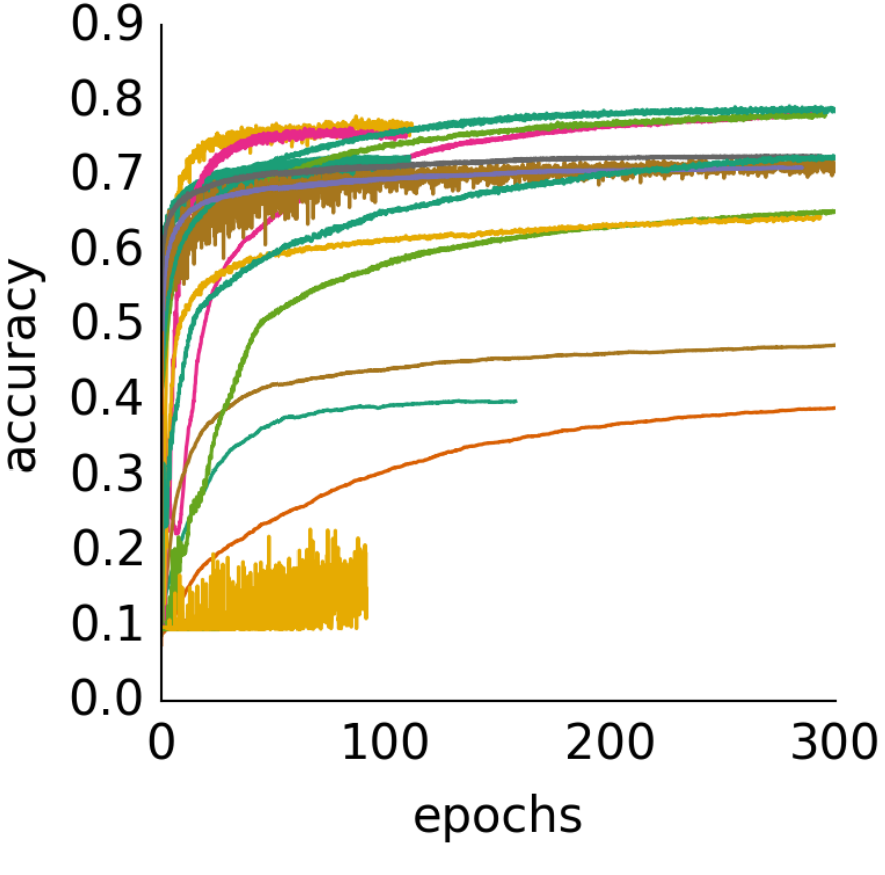
\includegraphics[width=0.5\textwidth]{images/learning_curves}

Exemplary learning curves of training deep neural networks\\
Many ML algorithms iteratively optimize a (loss) function

\end{frame}
%-----------------------------------------------------------------------

%-----------------------------------------------------------------------
\begin{frame}[c,fragile]{Learning Curve Predictions}

\centering
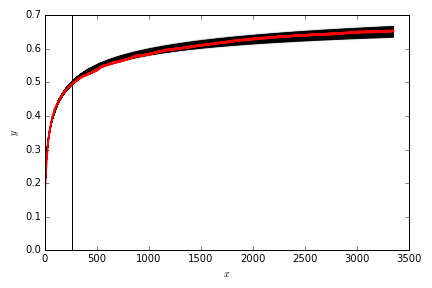
\includegraphics[width=0.6\textwidth]{images/learning_curve_single_pred}

\begin{enumerate}
  \item Observe learning curve for the first $n$ steps (here $n=250$)
  \pause
  \item Fit parametric model on partial learning curve to predict remaining learning curve
  \pause
  \item Which model to use? 
  \begin{itemize}
    \item Good model depends on shape of curve $\to$ e.$\,$g., depends on optimizer  
    \item[$\leadsto$] combination of several models
  \end{itemize}
  
\end{enumerate}

\end{frame}
%-----------------------------------------------------------------------

%-----------------------------------------------------------------------
\begin{frame}[c,fragile]{Learning Curves: Early Termination}

\centering
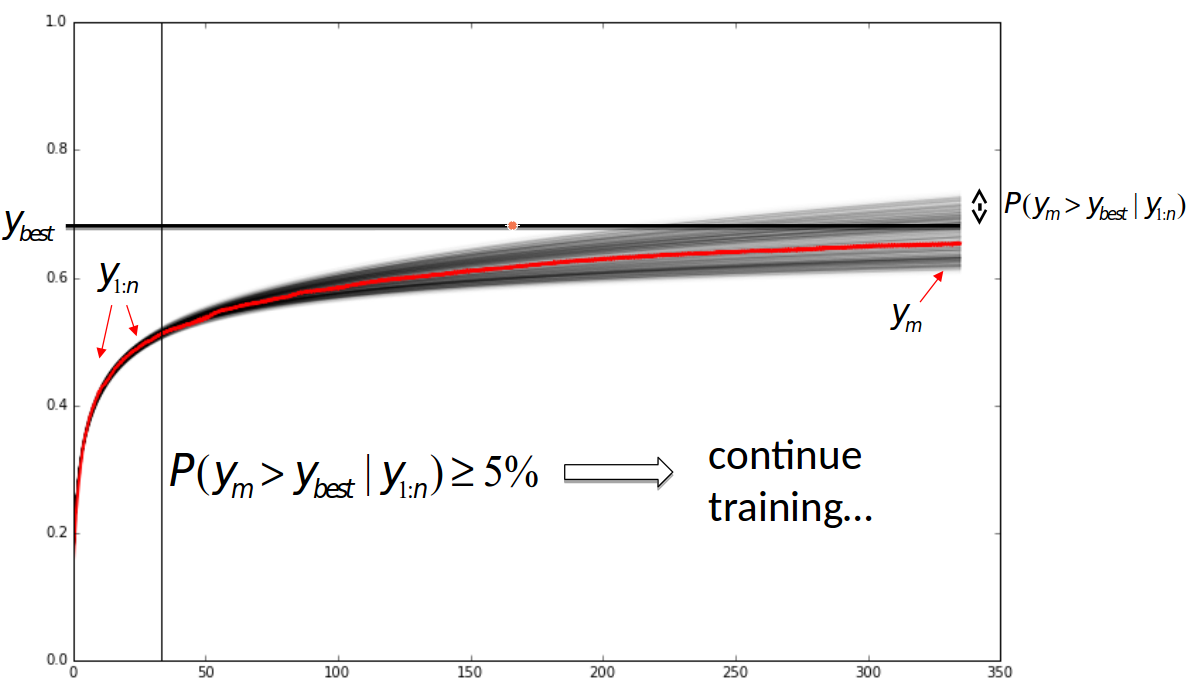
\includegraphics[width=\textwidth]{images/learning_curve_dec}

\end{frame}
%-----------------------------------------------------------------------
%-----------------------------------------------------------------------
\begin{frame}[c,fragile]{Learning Curves: Early Termination}

\centering
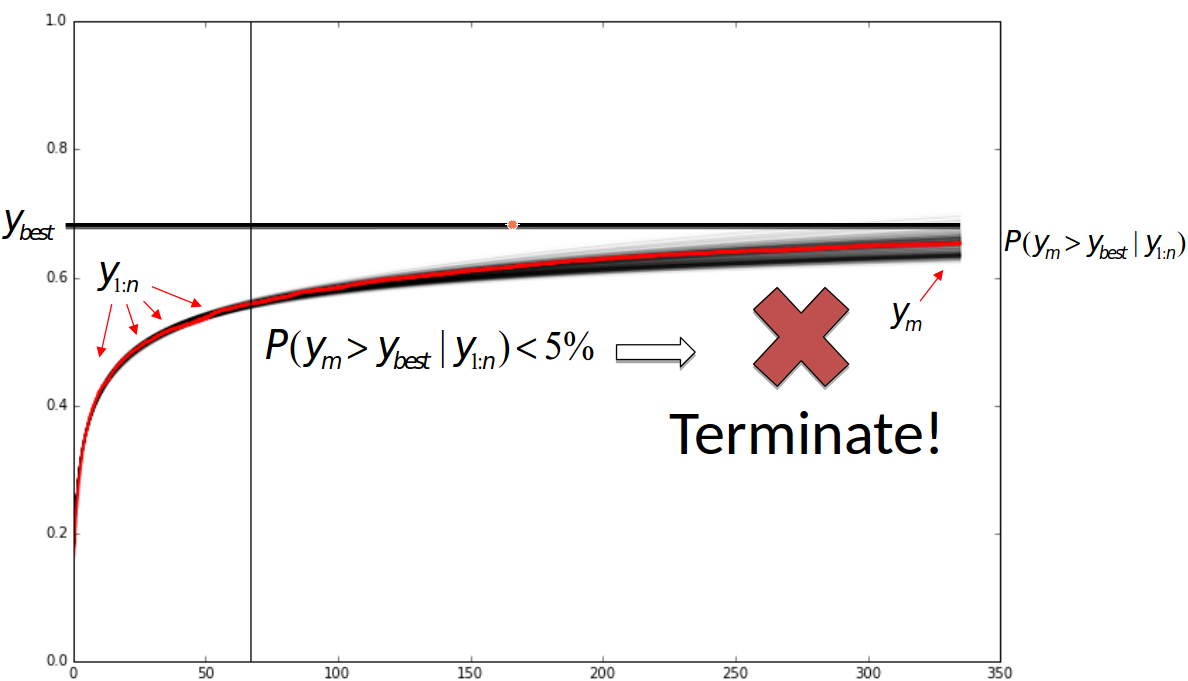
\includegraphics[width=\textwidth]{images/learning_curve_dec2}

\end{frame}
%-----------------------------------------------------------------------
%-----------------------------------------------------------------------
\begin{frame}[c,fragile]{Learning Curves: Early Termination}

\centering
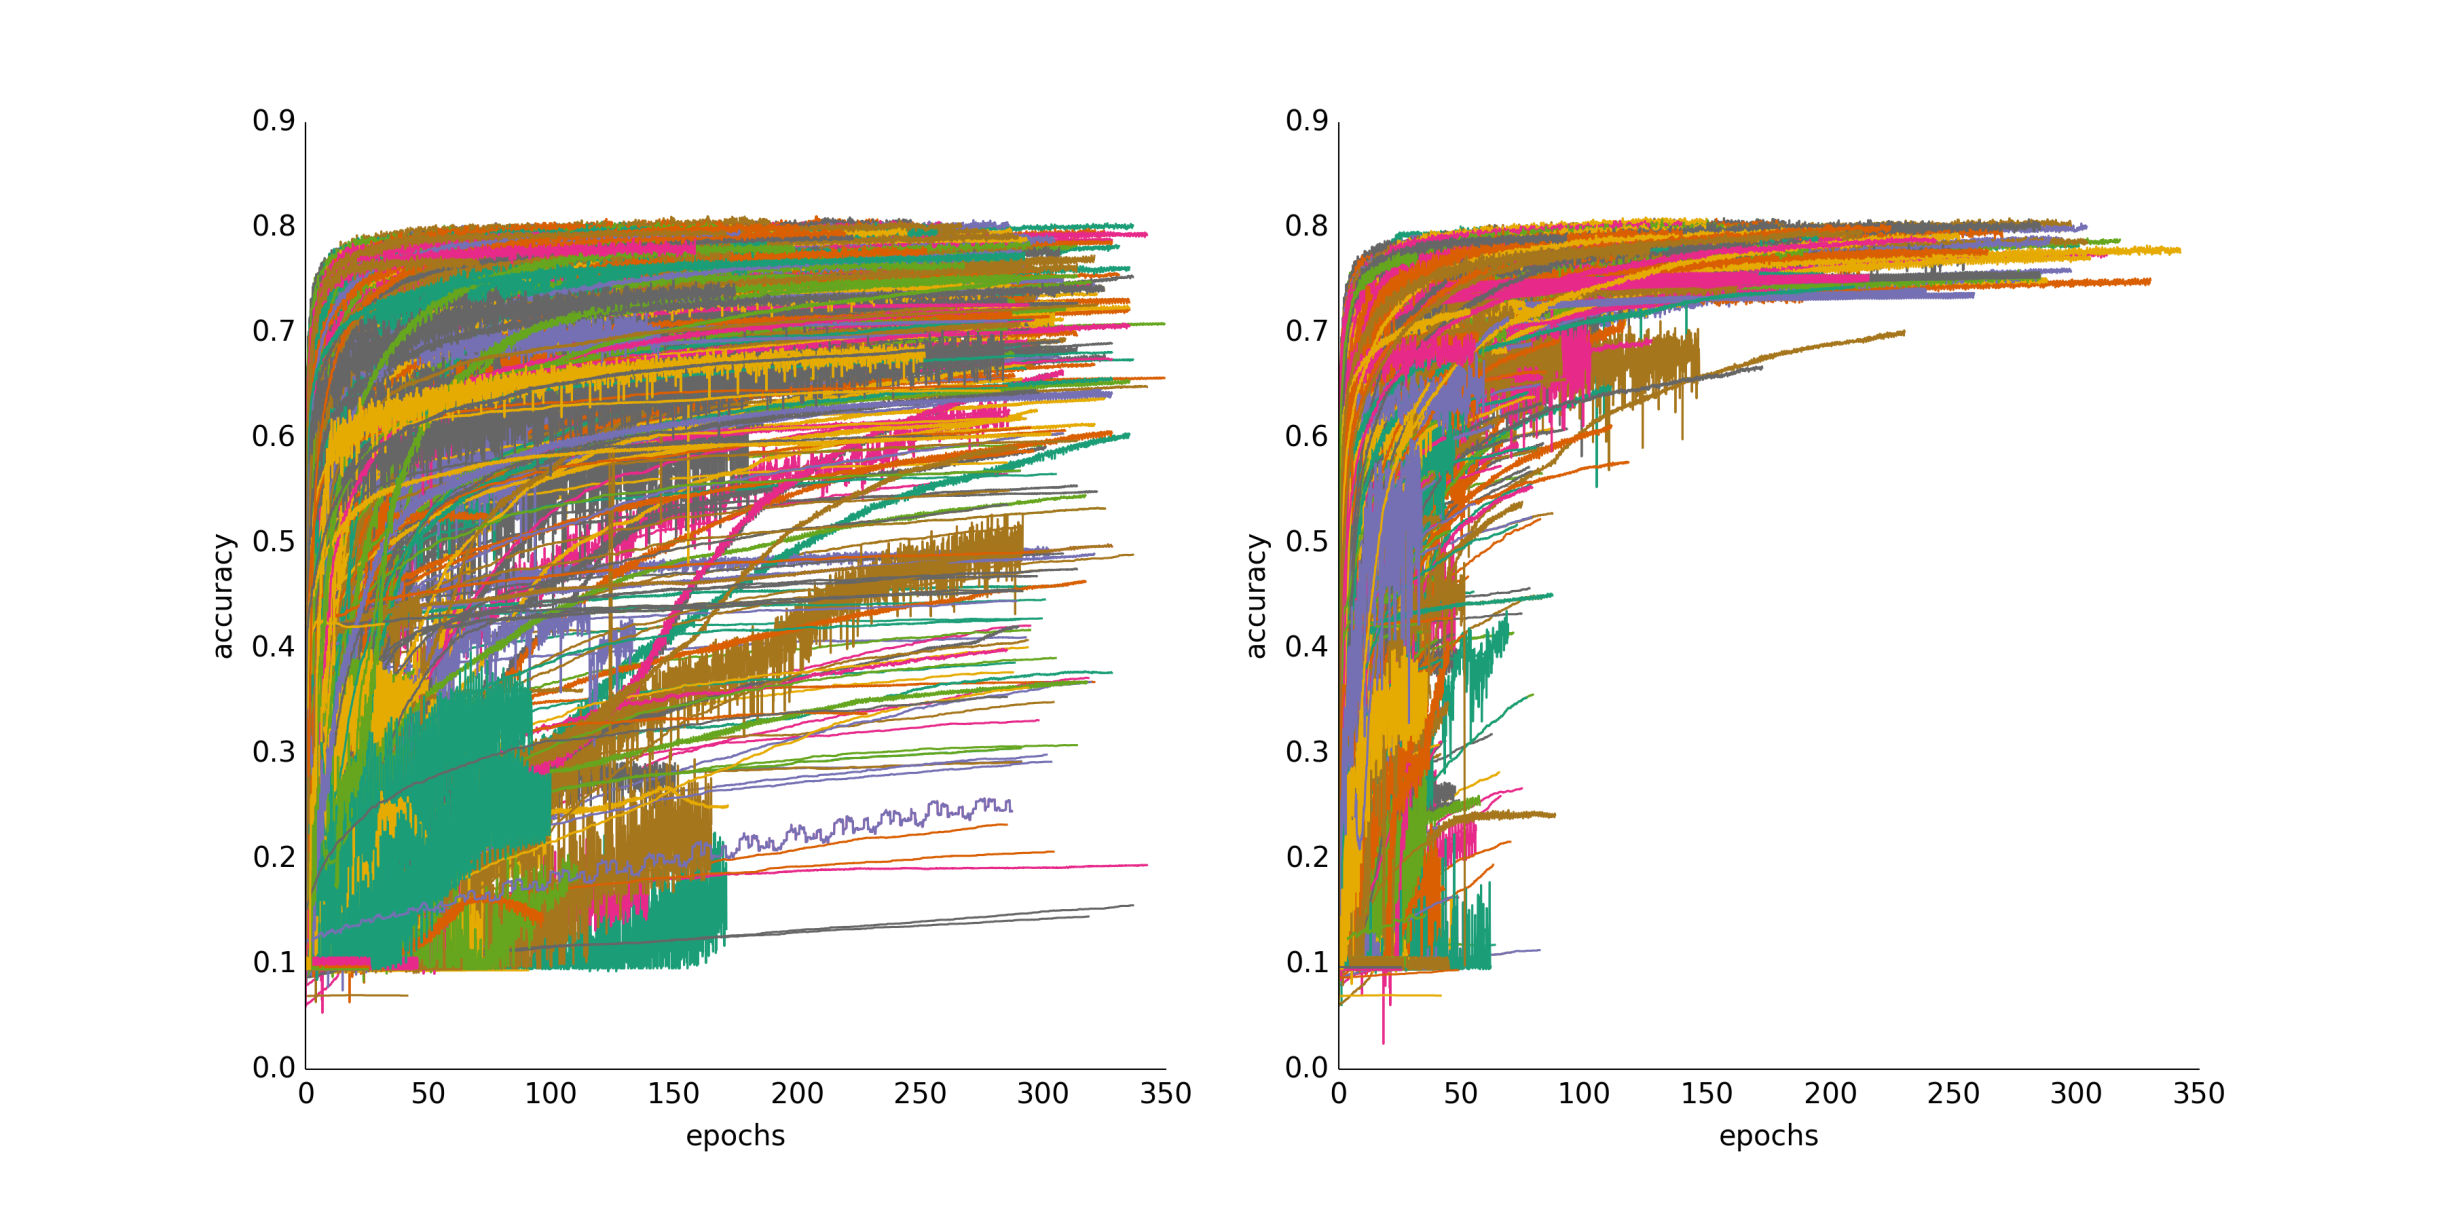
\includegraphics[width=\textwidth]{images/learning_curve_tuning}

All learning curves vs. Learning curves with early termination

\end{frame}
%-----------------------------------------------------------------------

%-----------------------------------------------------------------------
\begin{frame}[c,fragile]{Subset Selection \litw{Klein et al. 2017}}

\begin{itemize}
  \item Problem: training is very slow for large datasets
  \item Idea: scaling up from subsets of data
  \item Example SVM:
  \begin{itemize}
    \item Computational cost grows quadratically in dataset size $s$
    \item Error shrinks smoothly with $s$
    \item Two parameters: $C$, $\lambda$
  \end{itemize}
\end{itemize}

\centering
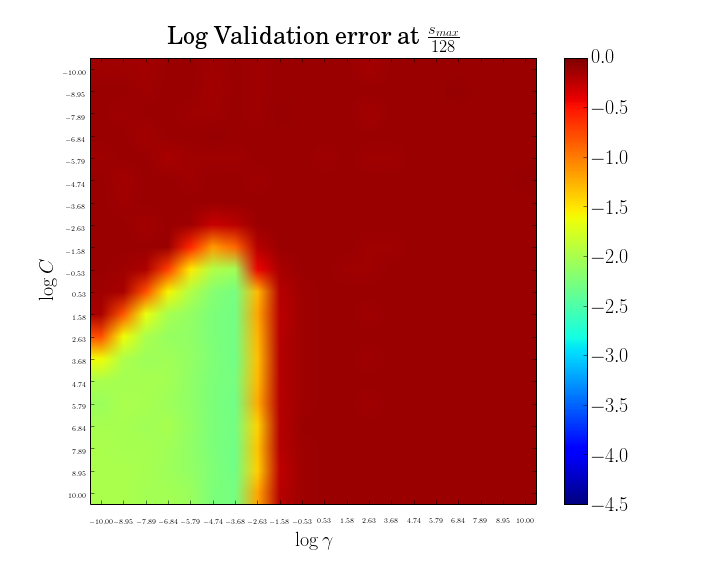
\includegraphics[width=0.28\textwidth]{images/subset_128}
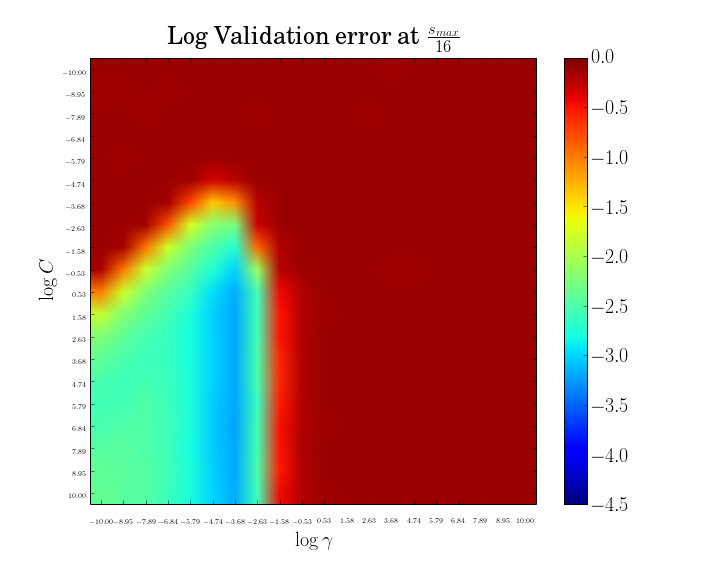
\includegraphics[width=0.28\textwidth]{images/subset_16}\\
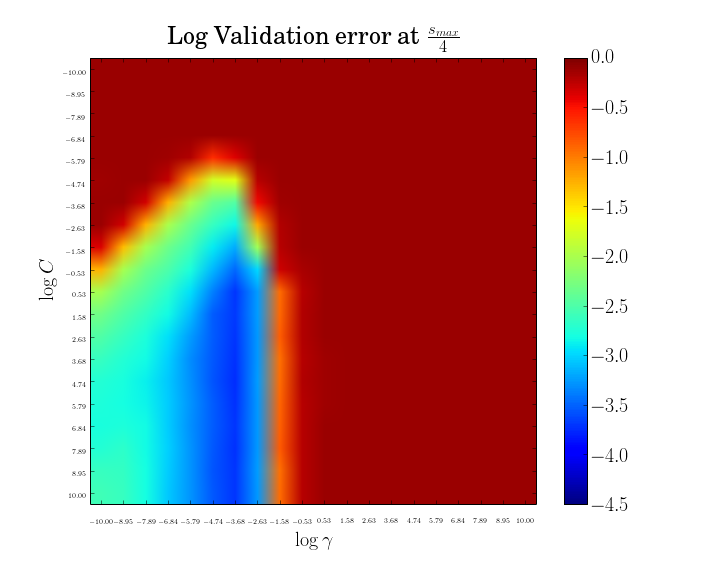
\includegraphics[width=0.28\textwidth]{images/subset_4}
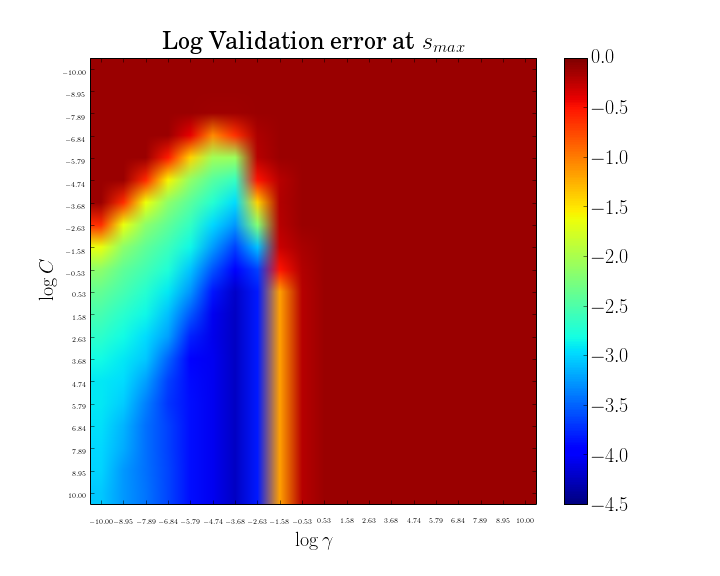
\includegraphics[width=0.28\textwidth]{images/subset_full}


\end{frame}
%-----------------------------------------------------------------------

%-----------------------------------------------------------------------
\begin{frame}[c,fragile]{Subset Selection \litw{Klein et al. 2017}}

\begin{itemize}
  \item Automatically choose dataset size for each evaluation
  \item Include extra dimension in probabilistic model to capture dependence on dataset size s: $f(\lambda,s)$
  \item Construct a second model for computational cost: $c(\lambda,s)$
  \item Trade off information gain about global optimum vs. cost
  \begin{itemize}
   \item Entropy Search \lit{Hennig \& Schuler, JMLR 2012}:\\ Based on a probability distribution of where the maximum lies
  \end{itemize} 
\end{itemize}

\centering
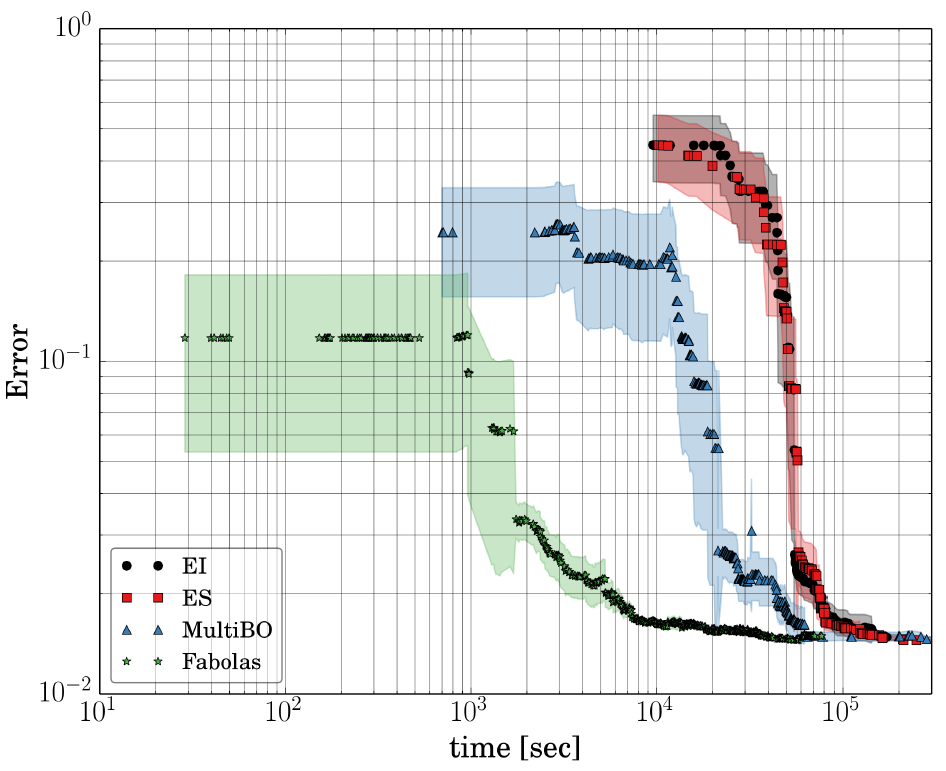
\includegraphics[width=0.4\textwidth]{images/subset_results}

\end{frame}
%-----------------------------------------------------------------------

%-----------------------------------------------------------------------
{\setbeamertemplate{logo}{}
\begin{frame}[c,fragile]{Successive Halving \litw{Jamieson and Talwalkar 2015}}

\begin{block}{Successive Halving}
\begin{itemize}
  \item Ideas: 
  \begin{itemize}
    \item Invest only resources in promising configurations
    \item[$\leadsto$] aggressive dropping of poor configurations
    \item Model-free --- (more or less assumption free)
  \end{itemize}
  \pause
  \item Algorithm Outline:
  \begin{enumerate}
    \item[-] Input: $n$ (randomly sampled) configurations and budget $B$
    \pause
    \item Run remaining configurations with some resource allocation\\ (depending on $B$)
    \pause
    \item Sort configurations by cost (e.$\,$g., validation loss)
    \item Throw away lower half of configurations
    \pause
    \item Repeat
  \end{enumerate}
  \pause
  \item Resource allocation can correspond to
  \begin{itemize}
    \item partial learning curves
    \item subset of training data
  \end{itemize}
\end{itemize}
\end{block}

\end{frame}
}
%-----------------------------------------------------------------------
%-----------------------------------------------------------------------
{\setbeamertemplate{logo}{}
\begin{frame}[c,fragile]{Hyperband \litw{Li et al. 2016}}

\begin{block}{Hyperband}
\begin{itemize}
  \item Issue of successive halving (for a fixed $B$):\\
  		Do you want to run many configurations with aggressive rejection?\\
  		Or: Do you want to run few configurations with non-aggressive rejection? 
  \pause
  \item Ideas: 
  \begin{itemize}
    \item Add an outer loop to try different trade-offs between $\#$configurations and budget
    \item Add further parameter: proportion of configurations discarded in each round of successive halving
  \end{itemize}
  \pause
  \item Starts with many configurations that gets aggressively rejected
  \pause
  \item In later iterations, few configurations with more budget each
  \pause
  \item Returns: configuration with the smallest intermediate loss seen so far.
\end{itemize}
\end{block}

\end{frame}
}
%-----------------------------------------------------------------------
%-----------------------------------------------------------------------
\begin{frame}[c,fragile]{Random Search vs. Hyperband}

\centering
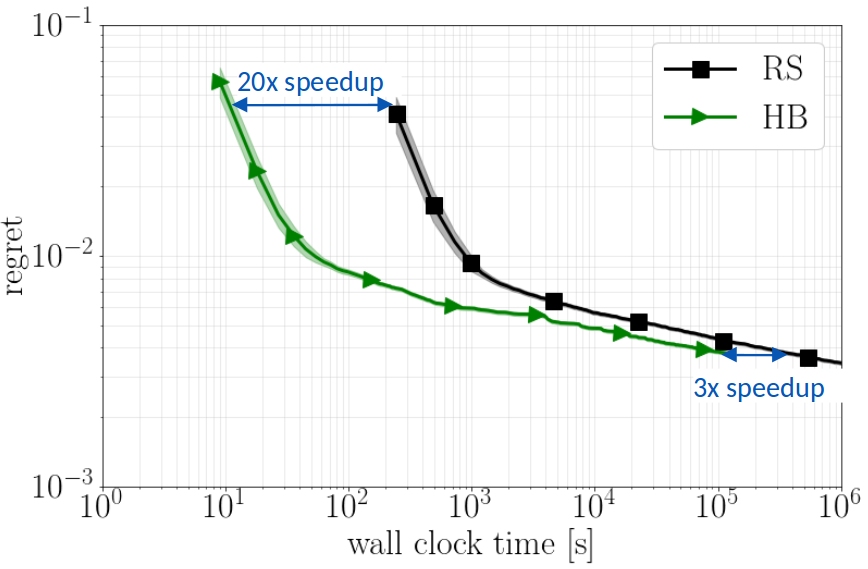
\includegraphics[width=0.8\textwidth]{images/randomsearch_hyperband}

\end{frame}
%-----------------------------------------------------------------------
%-----------------------------------------------------------------------
\begin{frame}[c,fragile]{Random Search vs. Bayesian Optimization}

\centering
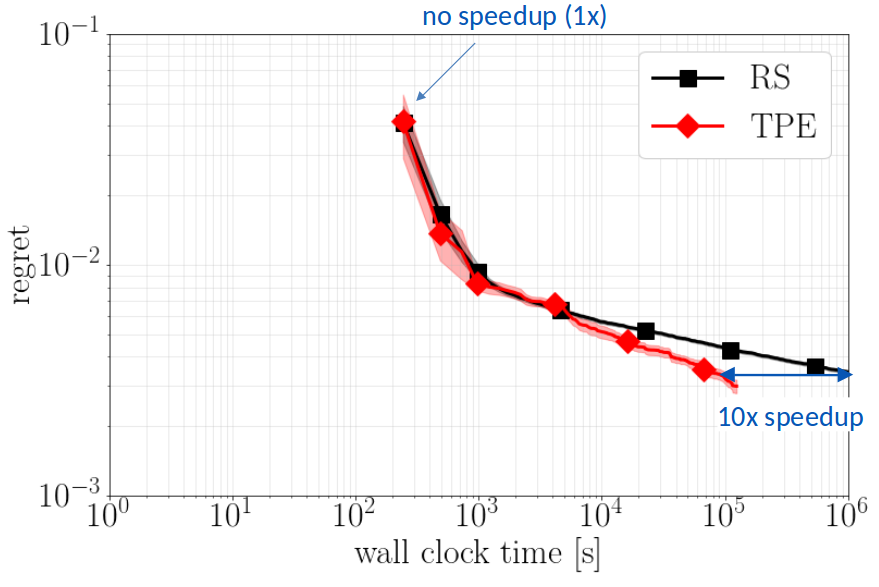
\includegraphics[width=0.8\textwidth]{images/randomsearch_bo}

\end{frame}
%-----------------------------------------------------------------------
%-----------------------------------------------------------------------
\begin{frame}[c,fragile]{Random Search vs. Bayesian Optimization vs. Hyperband}

\centering
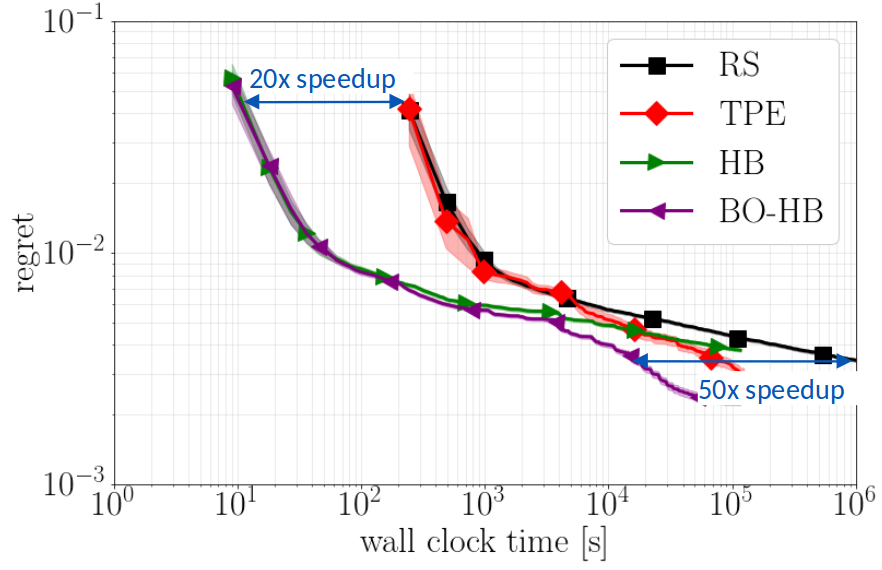
\includegraphics[width=0.8\textwidth]{images/randomsearch_bohb}

\end{frame}
%----------------------------------------------------------------------
